\documentclass{article}
\usepackage{blindtext}
\usepackage{csvsimple}
\usepackage{graphicx}
\usepackage{hyperref}


\title{NLP Project}
\author{Parsa Kangavari}
\begin{document} 
\maketitle

\section{Phase 1: Crawling And Cleaning Data}
Github Repository Link: \href{https://github.com/rezakongo/soccer_report_analyst}{Click here}.


\subsection{Step 1: Data Crawling}
At first we should find websites that include match reports and player's ratings of a match in a single pages. The best website for this is SkySport.
Then we should find and store urls of that pages. This urls has been crawled from a webpage that contains all matchs. For crawling we use Scrapy framework.
At first we should crawl all URLs from SkySport. So we should crawl urls from a page contains all urls. In this page there will be all urls of all matches.
We should choose seasions that we want. In this project we have chosen Primier league, Champions league and Fifa World Cup.

All matches page link: \href{https://www.skysports.com/premier-league-results}{Click here}.


Then we have been crawled urls of pages contains reports from this page and save them as a csv file. We have developed a spider that do this. you can see it in MatchURLSpider.py.

Results:
\begin{center}
\csvautotabular[]{urls.csv}
\end{center}


After that we have crawld reports and player ratings from each urls in dataset above. This informations have been crawld by a spider that you can see in SoccerSpider.py.
In this spider we read urls CSV file and then crawl all informations from each url.

Results: 
\begin{center}
\csvautotabular[]{row_data.csv}
\end{center}

\subsection{Setp 2: Cleaning Data}
For this section we have to clean datas that we crawled before. We should tokenize reports of matchs by sentences and words. 
For first one we split report by dots and for second one we split them by spaces. Then we should clean player ratings. player ratings are in range 0 to 10.
We should set ratings true if they are bigger than 6 and set false otherwise.

tokenized by sentences:
\begin{center}
\csvautotabular[]{sentence_broken_data.csv}
\end{center}
You can also see it on : \href{https://huggingface.co/datasets/ParsaKgvr/socce_report_analysis}{Click here}


tokenized by words:
\begin{center}
\csvautotabular[]{word_broken_data.csv}
\end{center}



\subsection{Step 3: Metrics}
For this section we should get most regular words, unique words of each reports and ... . At first we should create new datasets that contains of 
sentences that belongs to positive and negative players. We have done it in PandNSeperation.py. In this script we seperate sentences belong to negative players 
and positive players and then save them in 2 seperated CSV file; negative and positives.csv.
In this datasets, there are seperated sentences. 

Results for negative:
\begin{center}
\csvautotabular[]{negative_data.csv}
\end{center}

Results for positives:
\begin{center}
\csvautotabular[]{positive_data.csv}
\end{center}



Then we should get metrics from that datas. So we write a script thet get all metrics. In SeperatedDataGetMetrics.py all metrics of seperated datas
has been gotten. You can see all metrics as follow:
\begin{center}
\csvautotabular[]{metrics_seperared.csv}
\end{center}


top10CommonNegativeWordsFrequency:
\begin{center}
    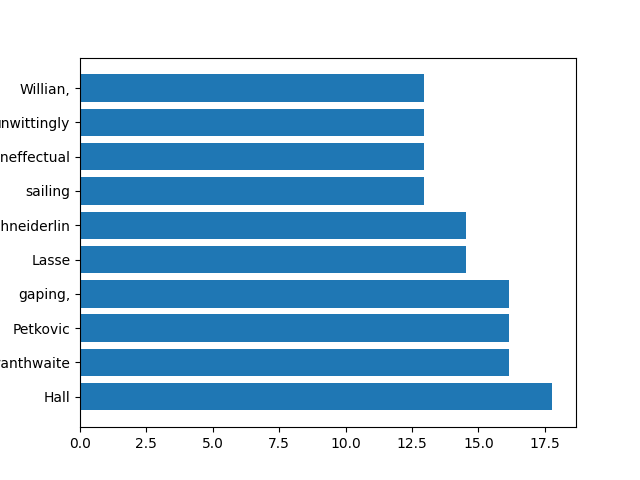
\includegraphics{top10CommonNegativeWordsFrequency}
\end{center}

top10CommonNegativeWordsTFIDF:
\begin{center}
    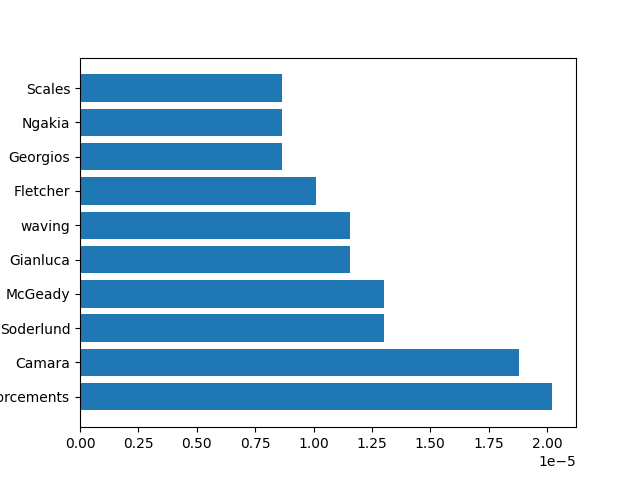
\includegraphics{top10CommonNegativeWordsTFIDF}
\end{center}

top10CommonPositiveWordsFrequency:
\begin{center}
    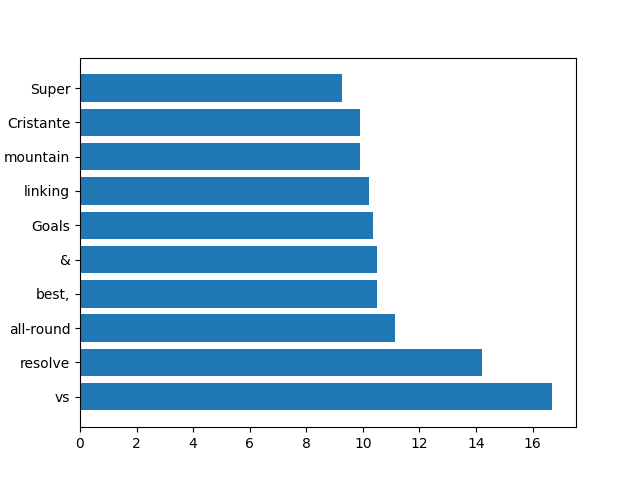
\includegraphics{top10CommonPositiveWordsFrequency}
\end{center}

top10CommonPositiveWordsTFIDF
\begin{center}
    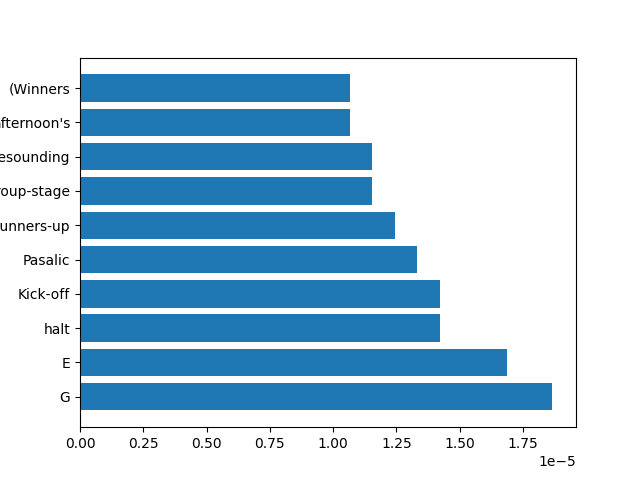
\includegraphics{top10CommonPositiveWordsTFIDF}
\end{center}

top10NegativeWordsCount
\begin{center}
    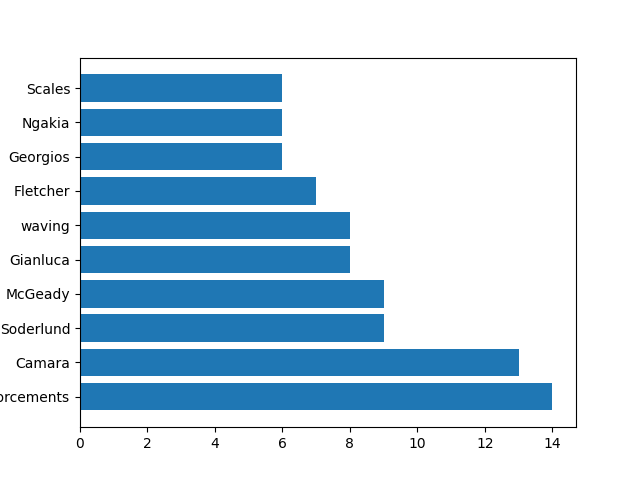
\includegraphics{top10NegativeWordsCount}
\end{center}

top10PositiveWordsCount
\begin{center}
    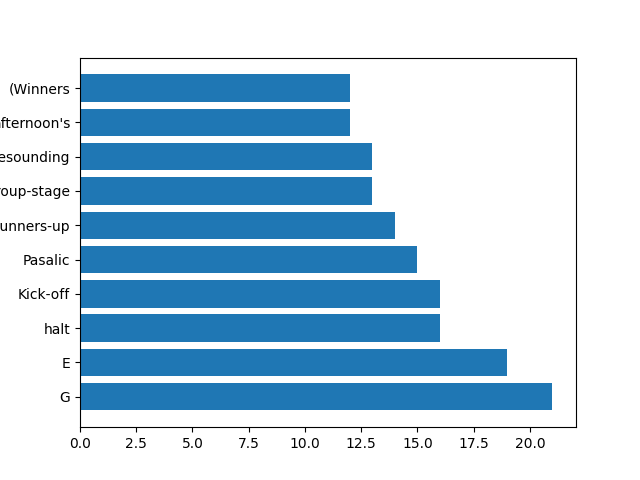
\includegraphics{top10PositiveWordsCount.png}
\end{center}

After that we should get metrics from new datasets. 
\section{Phase 2: Model Implimentation}
Note: This part has been done in google colab environment at the link below.
https://colab.research.google.com/drive/1Sg-9LCH0BUBljELWQ9AeB7iqsqaRaZCH
All results of the project are in this workstation.


\subsection{Installing and Importing Dependencies}
At the beginning we should install and import some libraries:
\begin{itemize}
    \item Sentence Transformer: Sentence Transformers is a Python library that provides pre-trained models for generating high-quality sentence embeddings. It enables you to convert sentences or text snippets into fixed-length numerical representations called embeddings, which capture the semantic meaning and contextual information of the input text.
    \item Sklearn: Scikit-learn (or sklearn for short) is a popular open-source machine learning library in Python. It provides a wide range of tools and algorithms for data preprocessing, feature selection, model training, evaluation, and prediction.
    \item Pandas: Pandas is a popular open-source data manipulation and analysis library for Python. It provides easy-to-use data structures and data analysis tools, making it useful for tasks such as data cleaning, transformation, and analysis.
    \item Numpy: NumPy is a powerful Python library for scientific computing and data manipulation. It stands for "Numerical Python." NumPy provides support for large, multi-dimensional arrays and matrices, along with a collection of mathematical functions to operate on these arrays efficiently.
\end{itemize}

\subsection{Preprocessing Sentence broken dataset}
Then we should load sentence broken dataset that we have built. Then we should make that dataset in form that be able to feed to our models.
For this goal, at first we seperate sentences about each player in each match. After that we have achived a dataset about players with label True and False.
Then we change lables from True and False into 0 and 1. In addition, we get sentence embeddings of sentences about each players.
After all, we have a dataset contains players'name, sentence embeddings of the player and his rating in the match.

\subsection{Feature Extraction}
Feature selection by clustering is a technique used to select a subset of relevant features from a larger set of available features in a dataset. It combines the principles of feature selection and clustering algorithms to identify the most informative features for a given task.

The process typically involves the following steps:
\begin{itemize}
    \item Clustering: Initially, a clustering algorithm like K-means, hierarchical clustering, or DBSCAN is applied to the dataset using all the available features. This step groups similar instances or data points together based on their feature values.
    \item Feature Importance Calculation: After clustering, a measure of feature importance is computed within each cluster. This measure can be based on various criteria such as intra-cluster variance, inter-cluster variance, or other distance measures. The goal is to determine which features contribute the most to the differences between clusters and have a high impact on the clustering result.
    \item Feature Ranking: Once the feature importance scores are calculated, the features are ranked based on their scores. The higher the score, the more important the feature is considered to be in distinguishing between clusters.
    \item Feature Selection: Finally, a subset of the top-ranked features is selected as the final set of features to be used for subsequent analysis or modeling tasks. Depending on the specific requirements, a threshold may be defined to determine the number or percentage of features to be selected.
\end{itemize}
The advantage of feature selection by clustering is that it takes into account the underlying patterns and relationships within the data to guide the selection process. By considering the information provided by the clustering algorithm, it aims to retain the most discriminative features while eliminating redundant or irrelevant ones. This can lead to improved efficiency, interpretability, and generalization performance of machine learning models.

For this goal at first, we have clustered all Sentence embeddings in the dataset into 50 clusters. Each cluster should be a feature of each player; And then feed sentence embeddings of each player into the kmeans model and get 50 features of him.
Finally we have 50 features of each player. Append these 50 features into the dataset and getting ready for feeding this dataset into a model for classification.

\subsection{Classification of players}
Sklearn, short for scikit-learn, is a popular machine learning library in Python that provides various algorithms and tools for classification, regression, clustering, and more. To perform classification using sklearn, you typically follow these steps:
\begin{itemize}
    \item Data Preparation: Firstly, you need to prepare your dataset by splitting it into input features X and target variable y. X represents the independent variables/features, while y represents the dependent variable/class labels you want to predict.
    \item Train and Test Split: It is common practice to split your dataset into training and testing subsets. The training set is used to train the classifier, while the testing set is used to evaluate its performance on unseen data.
    \item Choose a Classifier: Select an appropriate classifier algorithm from sklearn based on your problem requirements. Sklearn offers various classification algorithms such as Logistic Regression, Support Vector Machines, Random Forest, etc.
    \item Instantiate and Train: Create an instance of the chosen classifier and then fit/train it on the training data using the fit method. This step involves learning the patterns and relationships between the features and class labels.
    \item Prediction: Once the classifier is trained, you can use it to make predictions on new, unseen data. Use the predict method or related methods of the classifier to generate predictions based on the learned model.
    \item Evaluate Performance: Compare the predicted class labels with the actual class labels of the test set to evaluate the performance of your classifier.
\end{itemize}

We should classify all players by their 50 features in 2 classes. We use sklearn linear model to do this. First 1900 entries are datas for train and last 100 datas are datas for test. 
All 50 features are X and rating is Y.

\subsection{Finalizing Project}
Finally we have 3 trained models:
\begin{itemize}
    \item Sentence Transformer: This model gets a list of sentences and give the list of embeddings of that sentences.
    \item Clustering Model: This model gets a list of Sentence embeddings and give the cluster of that sentences. This model is being used for feature Extraction of players.
    \item Classification Model: This model gets features of a player and classify that player.
\end{itemize}

Here is Final Model:
\begin{center}
    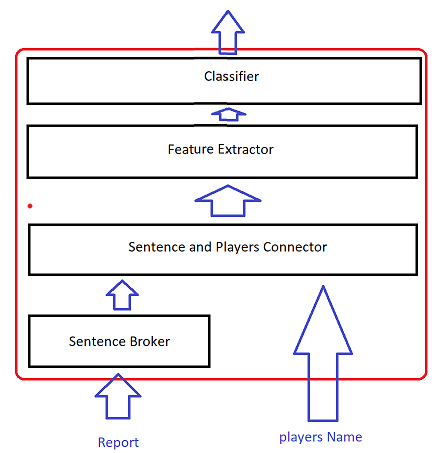
\includegraphics{FinalModel.png}
\end{center}

This model gets report and 22 players name of a match. Then it breaks sentences for each player and then gets their embeddings. After that it Extracts 50 features of each players.
Finally it classify players by their features.

\end{document}